% =====================================================================
\section{Spatial, temporal and environmental context}\label{sec:context}

\subsection{Spatial variation}
Test forecasts were aggregated by origin on a \ang{1} grid, keeping cells with at least 100 forecasts from at least three distinct drifters. This retains 145 of 198 occupied cells and \num{73214} forecasts (88.7\%) (\cref{fig:spatial}). Because the split was by drifter, not by location, test drifters pass through the same areas as training drifters. The maps therefore describe \emph{where} the model is more or less accurate; they do not test generalisation to unseen regions.

\begin{figure}[!htbp]
  \centering
  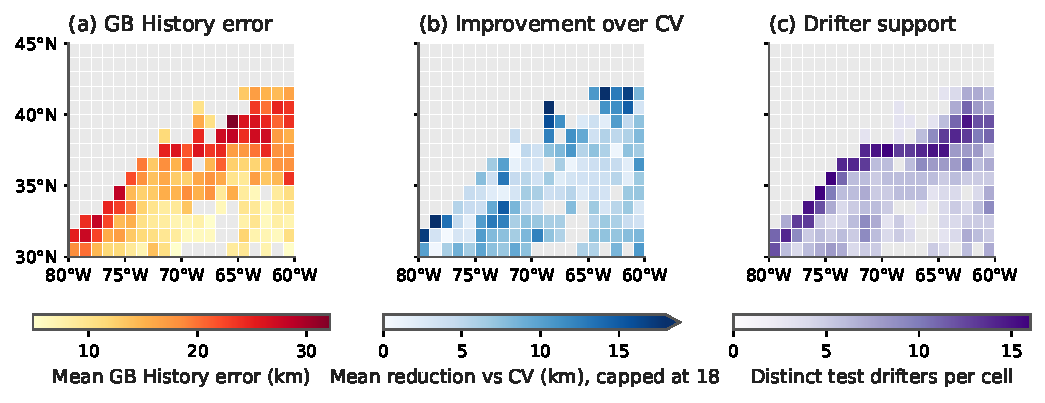
\includegraphics[width=\textwidth]{figures/generated/fig_spatial_performance_rescaled.pdf}
  \caption{Spatial variation in held-out performance (cells with $\ge$100 forecasts and $\ge$3 drifters; grey: excluded or unsampled). (a) Mean \GBH{} error. (b) Mean reduction in error relative to CV. The colour scale is capped at \SI{18}{km} (98th percentile of cell values) for readability; three cells exceed it: \SI{42.0}{km} at \ang{40}N\,\ang{69}W (3 drifters), \SI{20.4}{km} at \ang{32}N\,\ang{79}W and \SI{18.5}{km} at \ang{41}N\,\ang{64}W (cells labelled by south-west corner). No cell has a negative mean reduction. (c) Distinct test drifters per cell. Re-plotted from saved test predictions with the notebook's aggregation rules, which were verified to reproduce its 145 cells and \num{73214} forecasts; the original figure used a symmetric \SI{\pm 42}{km} scale set by the single largest cell.}
  \label{fig:spatial}
\end{figure}

Absolute difficulty is spatially structured. Mean \GBH{} errors exceed \SI{25}{km} in a band running from the south-western corner of the box north-eastward to about \ang{38}--\ang{40}N, \ang{60}--\ang{68}W. The worst cell (\ang{39}N\,\ang{66}W) averages \SI{32.2}{km} but rests on only three drifters. Errors are below \SI{10}{km} in much of the south-central box. The high-error band broadly follows the region where one would expect the Gulf Stream jet and its extension, and it coincides with the cells of highest drifter support (\cref{fig:spatial}c). We did not overlay an independent current-axis product, however, so this correspondence remains qualitative.

The \emph{improvement} over CV is positive in all 145 cells (median \SI{6.2}{km}, minimum \SI{0.3}{km}), so the advantage of the learned correction is not confined to a sub-region. High-error cells are not necessarily cells of low improvement. For example, the cell at \ang{38}N\,\ang{67}W combines a \SI{27.3}{km} mean error with an \SI{11.3}{km} improvement, whereas the cell at \ang{39}N\,\ang{64}W improves by only \SI{1.9}{km}. Cell estimates are noisy, because most cells rest on 3--10 drifters (median 6) whose forecasts are strongly autocorrelated, and individual cells should not be over-interpreted.

\subsection{Temporal stability}
\GBH{} had the lowest median error of the three compared methods (CV, \GBC, \GBH) in every one of the 16 years, and \GBC{} beat CV in every year. Annual \GBH{} medians ranged from \SI{6.5}{km} (2013) to \SI{16.0}{km} (2009), but each year contains only 3--13 test drifters, so year-to-year variation largely reflects which drifters happen to be present. Aggregated into four periods (\cref{tab:temporal}), the advantage is remarkably stable. The mean reduction relative to CV is \SIrange{7.1}{7.8}{km} and the mean benefit of history \SIrange{3.4}{4.2}{km} in every period. Because training and test drifters cover the same years, this shows temporal consistency within 2007--2022, \emph{not} prospective skill in future years.

\begin{table}[!htbp]
\centering
\caption{Test performance by period (km). Gains are mean paired reductions. Drifters may contribute to more than one period. Source: notebook cell 63; yearly values are plotted in \cref{fig:temporal}.}
\label{tab:temporal}
\small
\begin{tabular}{@{}lrrrrrrr@{}}
\toprule
 & & & \multicolumn{3}{c}{Median error} & \multicolumn{2}{c}{Mean gain of \GBH} \\
\cmidrule(lr){4-6}\cmidrule(lr){7-8}
Period & Cases & Drifters & CV & \GBC & \GBH & vs CV & vs \GBC \\
\midrule
2007--2010 & \num{18316} & 22 & 15.63 & 13.57 & 9.46 & 7.12 & 4.20 \\
2011--2014 & \num{27654} & 30 & 15.42 & 12.40 & 8.77 & 7.29 & 3.36 \\
2015--2018 & \num{20056} & 14 & 16.92 & 13.67 & 10.10 & 7.12 & 3.48 \\
2019--2022 & \num{16520} & 15 & 15.71 & 12.84 & 8.85 & 7.82 & 3.73 \\
\bottomrule
\end{tabular}
\end{table}

\begin{figure}[!htbp]
  \centering
  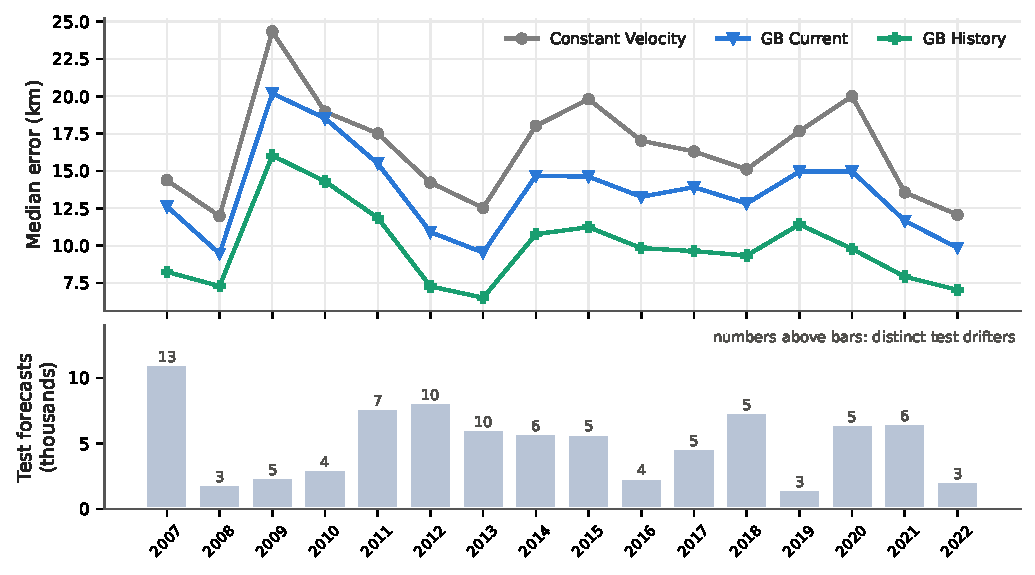
\includegraphics[width=0.9\textwidth]{figures/generated/fig_temporal.pdf}
  \caption{Median test error by year for CV, \GBC{} and \GBH{} (top), and the number of test forecasts and distinct test drifters per year (bottom). Several years rest on three to five drifters. Re-plotted from saved test predictions; values reproduce notebook cell 63.}
  \label{fig:temporal}
\end{figure}

\subsection{Sea-surface temperature: association versus predictive value}
SST is an environmental variable rather than a kinematic one, so we examined it in two distinct ways.

\paragraph{SST as a descriptive stratifier.} Using training-tertile thresholds (\SIlist{26.93;28.06}{\celsius}) on the \num{77845} test forecasts with origin SST, errors decrease from the Low to the High SST regime for all three methods (\cref{fig:sst}a--c): \GBH{} medians are \SIlist{9.98;9.28;8.28}{km} and CV medians \SIlist{17.59;15.50;14.93}{km}. The mean benefit of history is slightly larger at Low SST (\SI{4.09}{km} against \SIlist{3.49;3.39}{km}), although median benefits are almost identical (\SIrange{3.34}{3.47}{km}). SST is confounded with speed: High-speed forecasts make up 43.5\% of the Low-SST regime and about 40\% of the others, while Low-speed forecasts are most common at High SST (35.8\% against 24.4\%) (\cref{fig:sst}d). Within speed tertiles the SST gradient persists at low speed (\SI{6.44}{}$\to$\SI{4.81}{km}) and medium speed (\SI{8.61}{}$\to$\SI{7.57}{km}) but essentially vanishes at high speed (\SIrange{14.96}{15.77}{km}). SST is also tied to location and water mass (the Low regime has mean \SI{24.2}{\celsius} against \SI{28.8}{\celsius} for High), so these patterns cannot be attributed to temperature itself.

\begin{figure}[!htbp]
  \centering
  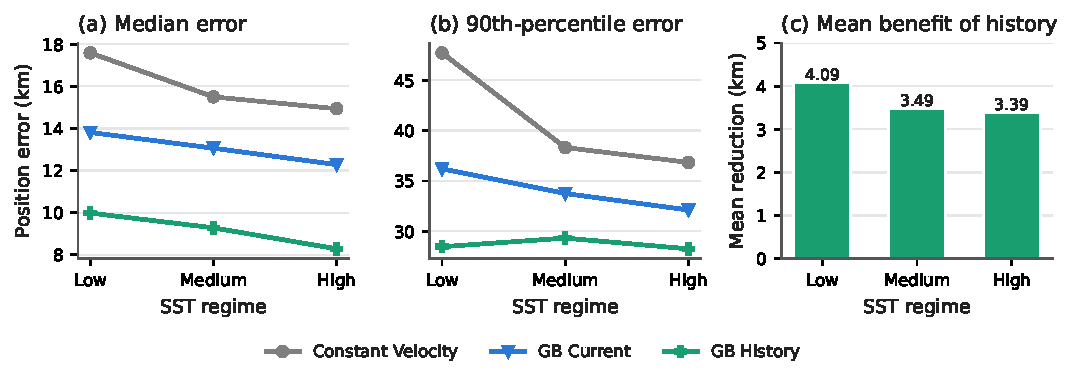
\includegraphics[width=\textwidth]{figures/generated/fig_sst_regimes.pdf}\\[2pt]
  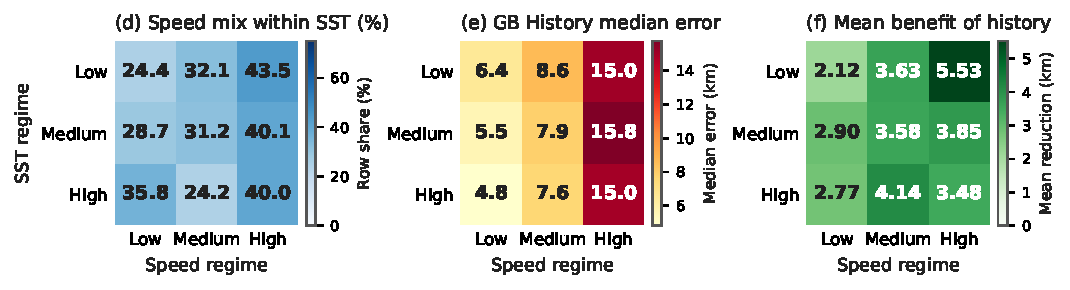
\includegraphics[width=\textwidth]{figures/generated/fig_sst_speed.pdf}
  \caption{SST-conditioned test performance (\num{77845} forecasts with origin SST). (a--c) Median and P90 error and mean benefit of history by SST regime. (d--f) Joint SST--speed regimes: speed mix within each SST regime (row \%), \GBH{} median error, and mean benefit of history. Descriptive associations only. Re-plotted from saved outputs; values reproduce notebook cells 68 and 70.}
  \label{fig:sst}
\end{figure}

\paragraph{SST as an additional predictor.} To test whether SST adds information \emph{beyond} kinematics, \GBH{} was refitted with origin SST as a 26th feature, keeping the hyperparameters, data and targets identical, and evaluated on the validation set (\cref{tab:sst}). The changes are negligible and mixed: the mean falls by \SI{0.019}{km} (0.16\%) and P90 by \SI{0.05}{km}, but the median rises by \SI{0.03}{km}. Only 50.1\% of individual forecasts improve, and the median paired change is \SI{0.002}{km}. Under this configuration, a single instantaneous SST value carries no useful additional predictive information. One possible explanation is that what SST says about the flow regime is already captured by position, velocity and recent motion. A richer representation, such as SST gradients or fronts, might behave differently. Because this experiment was run after the test set had been examined, it is reported as exploratory validation evidence.

\begin{table}[!htbp]
\centering
\caption{SST feature ablation on the validation set (\num{88471} forecasts, km). Source: notebook cell 74.}
\label{tab:sst}
\small
\begin{tabular}{@{}lrrrr@{}}
\toprule
Model & Mean & Median & P90 & RMSE \\
\midrule
\GBH{} (25 features)        & 11.969 & 8.507 & 24.977 & 16.681 \\
\GBH{} + SST (26 features)  & 11.950 & 8.537 & 24.929 & 16.633 \\
\bottomrule
\end{tabular}
\end{table}
